%
% hbars.tex
%
\section{Chart::HorizontalBars}
\name{Chart::HorizontalBars}
\file{HorizontalBars.pm}
\requires{Chart::Base, GD, Carp, FileHandle}
\begin{Description} 
\class{HorizontalBars} is a subclass of \class{Chart::Base}.\\
The class \class{HorizontalBars} creates a chart with bars, that run horizontal.
\end{Description}

\parindent 0pt{\large Example:}

\begin{figure}[h]
	\begin{center}
		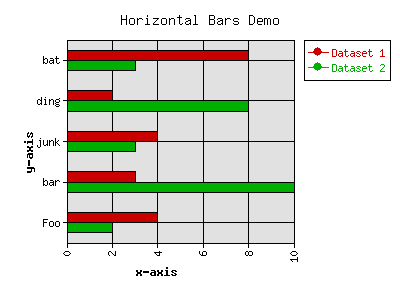
\includegraphics[scale=0.7]{d_hbars4.png}
	\end{center}
	\caption{Chart with horizontal bars}
	\label{fig:hbars}
\end{figure}
\begin{verbatim}
use Chart::HorizontalBars;

$g = Chart::HorizontalBars->new();
$g->add_dataset ('Foo', 'bar', 'junk', 'ding', 'bat');
$g->add_dataset (4, 3, 4, 2, 8);
$g->add_dataset (2, 10, 3, 8, 3);

%hash = ( 'title' => 'Horizontal Bars Demo',
          'grid_lines' => 'true',
          'x_label' => 'x-axis',
          'y_label' => 'y-axis',
          'include_zero' => 'true',
          'x_ticks' => 'vertical',
         );
$g->set (%hash);

$g->png ("hbars.png");
\end{verbatim}

\begin{Constructor} 
An instance of a HorizontalBars object can be created with the constructor new():
\begin{quote}
\parindent 0pt
\fett{\$obj = Chart::HorizontalBars->new();}\\
\fett{\$obj = Chart::HorizontalBars->new(\parameter{width}, \parameter{height});}
\end{quote}

If \textit{new()} has no arguments, the constructor returns an image with the size 300x400 pixels.
If \textit{new()} has two arguments \parameter{width} and \parameter{height}, 
it returns an image with the desired size.
\end{Constructor}

\Methods
\method{All universal valid methods, see page \pageref{methods}: Chart::Base.}\\[\parabstand]
%
\Attributes
All universally valid options, see page \pageref{options}. Also available, these special options:
\begin{description}
\item['y\_axes'] Tells chart where to place the y-axis. 
      Valid values are 'left', 'right' and 'both'. Defaults to 'left'.

\item['spaced\_bars'] Leaves space between the groups of bars 
     at each data point when set to 'true'.  
     This just makes it easier to read a bar chart.  Default is 'true'.

\item['skip\_y\_ticks'] 
     Does the same fo the y-axis at a HorizontalBars chart as 'skip\_x\_ticks' 
     does for other charts. Defaults to 1.
\end{description}
